\section{Diskretizacija problema}

Za reševanje problema z računalnikom moramo abs\-trakt\-no zastavitev \eqref{eq:LsfemVariationalStatement} z neskončno prostostnimi stopnjami narediti oprijemljivejšo. Domena $\Omega$ namreč kljub omejenosti vsebuje neskončno število točk, v katerih funkcijam dopuščamo neodvisne vrednosti. Število prostostnih stopenj omejimo tako, da poljubno funkcijo $v(\mathbf{x})$ razvijemo v vrsto $N$ baznih funkcij, ki jih izberemo sami:
\begin{IEEEeqnarray*}{rc}
    \hspace{16mm} \Phi_i(\bm\chi) \, , \hspace{5mm} i = 1, ..., N \hspace{16mm} & \texttt{vozliščne funkcije ,}
\end{IEEEeqnarray*}

Vzemimo skrajno preprosto kvadratno domeno $[-3,\mkern2mu 3\mkern1mu] \mkern-1mu \times \mkern-1mu [-3,\mkern2mu 3\mkern1mu]$ s krajevnim vektorjem $\bm{\chi} = \{\xi,\eta\}$. Nanjo postavimo pravokotno mrežo z $n$ (= 9) \textbf{elementi} in $N$ (= 16) \textbf{vozlišči} (slika \ref{fig:regionAndNodeFunctions}a). Nad vozlišči napnimo prav toliko vozliščnih funkcij:

z nastavljivo višino (\textbf{vozliščno vrednostjo}) $v_i\mkern1mu$ (slika \ref{fig:regionAndNodeFunctions}b).

Poljubno skalarno funkcijo $v(\mathbf{x})$ na domeni nato aproksimiramo s sestavljanko $N$ vozliščnih funkcij:
\begin{equation}
    v(\mathbf{x}) = \sum_{i = 1}^N v_i  \mkern3mu \Phi_i(\mathbf{x}) \ .
    \label{eq:nodalSeries}
\end{equation}

\begin{figure}[ht]
    \begin{subfigure}[b]{0.42\textwidth}
        \centering
        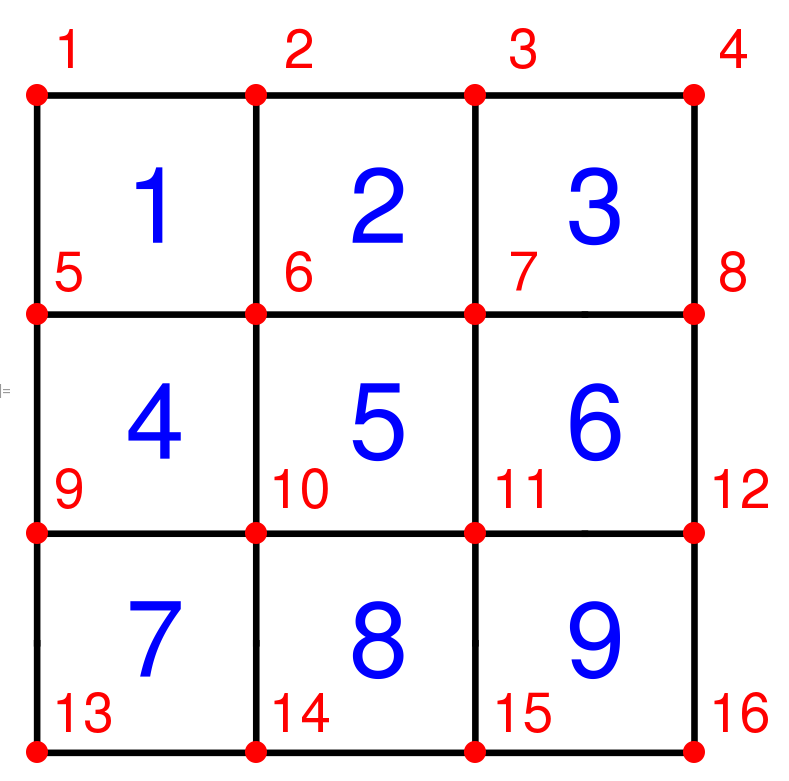
\includegraphics[height=67mm]{Slike/undeformedRegion.png}
        \vspace{6mm}
        \caption{}
    \end{subfigure}
    \begin{subfigure}[b]{0.55\textwidth}
        \centering
        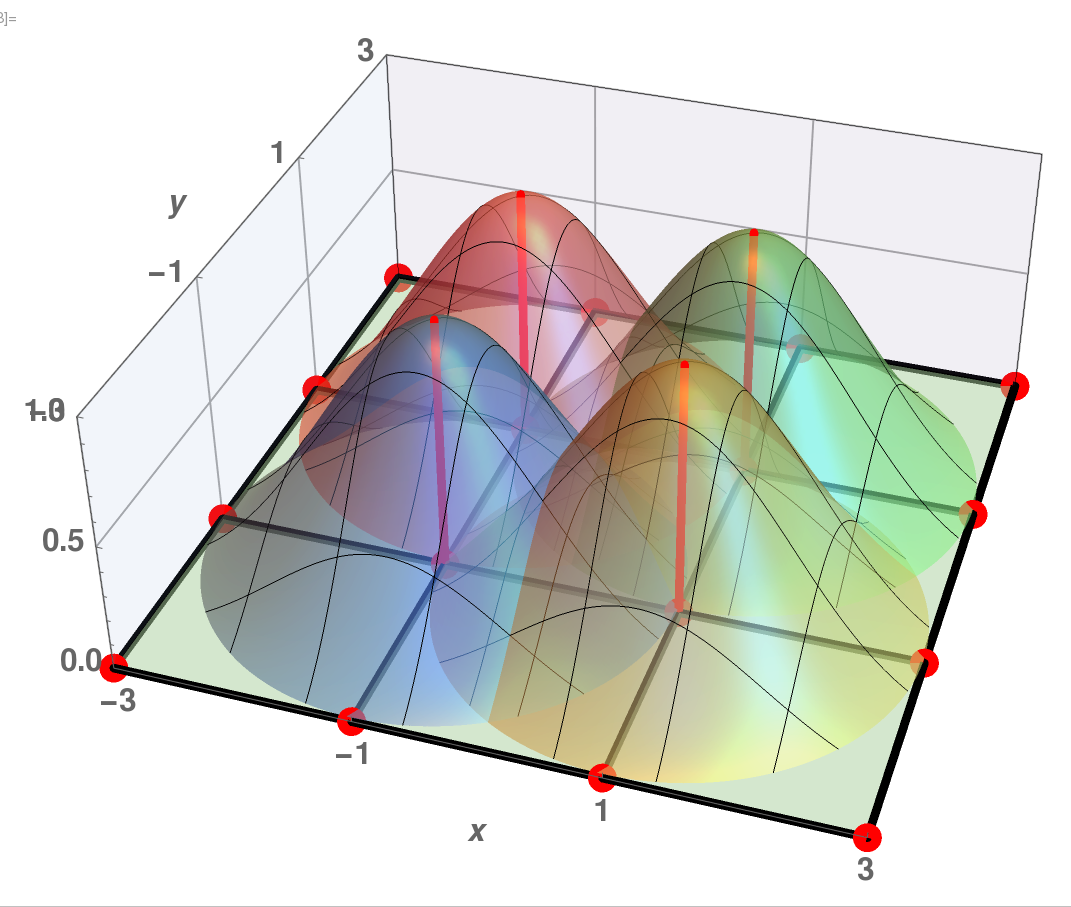
\includegraphics[width=0.94\textwidth]{Slike/undeformedNodeFs.png}
        \caption{}
    \end{subfigure}
    \caption{(a) Pravokotna domena z devetimi elementi (modre številke) in šestnajstimi vozlišči (rdeče številke) ter (b) nad vozlišči napete vozliščne funkcije. V prid nazornosti rišemo le osrednje vozliščne funkcije.}
    \label{fig:regionAndNodeFunctions}
\end{figure}

Nobena vozliščna funkcija $\Phi_i$ se ne sme raztezati nad elementi, ki niso v stiku z njenim vozliščem. S tem dosežemo, da je $v(\bm\chi)$ nad nekim elementom sestavljena le iz funkcij v neposredni bližini tega elementa. Tako je $\mathbf{v}(\bm\chi)$ na sliki \ref{fig:sumAndShapeFunctions}a nad osrednjim elementom popolnoma določena z vrednostmi $v_6, v_7, v_{10}$ in $v_{11}$.

Ozrimo se na variacijsko izjavo \eqref{eq:LsfemVariationalStatement} ter si predstavljajmo funkcije $\mathbsf{A}(\mathbf{x}), \mathbf{u(x)}, \mathbf{v(x)}$ in $\mathbf{f(x)}$ zapisane v smislu razvoja po vozliščnih funkcijah \eqref{eq:nodalSeries}. Zaslutimo, da bomo računali prekrivne integrale vozliščnih funkcij:
\begin{equation}
    \int \mkern-2mu \Phi_i(\mathbf{x}) \mkern4mu \Phi_j(\mathbf{x}) \mkern4mu \ud \Omega \ .
\end{equation}
To je enostavno dokler so vsi elementi iste oblike in velikosti, kot na sliki \ref{fig:regionAndNodeFunctions}. Takrat je dovolj, da izračunamo prekrivne integrale za vozlišča enega elementa. Kaj pa, če želimo uporabljati elemente poljubne oblike? Kako naj čim učinkoviteje, če so elementi poljubne oblike

 Segmente vozliščnih funkcij $\Phi_6, \, \Phi_7, \, \Phi_{10}$ in $\Phi_{11}$, ki se nahajajo neposredno nad elementom 5, proglasimo za \textbf{elementarne funkcije} $\phi_{5 j}(\bm\chi)$ tega elementa (slika \ref{fig:sumAndShapeFunctions}b). Tako lahko funkcijo $\mathbf{v}$ na

\begin{figure}[ht]
    \begin{subfigure}[b]{0.48\textwidth}
        \centering
        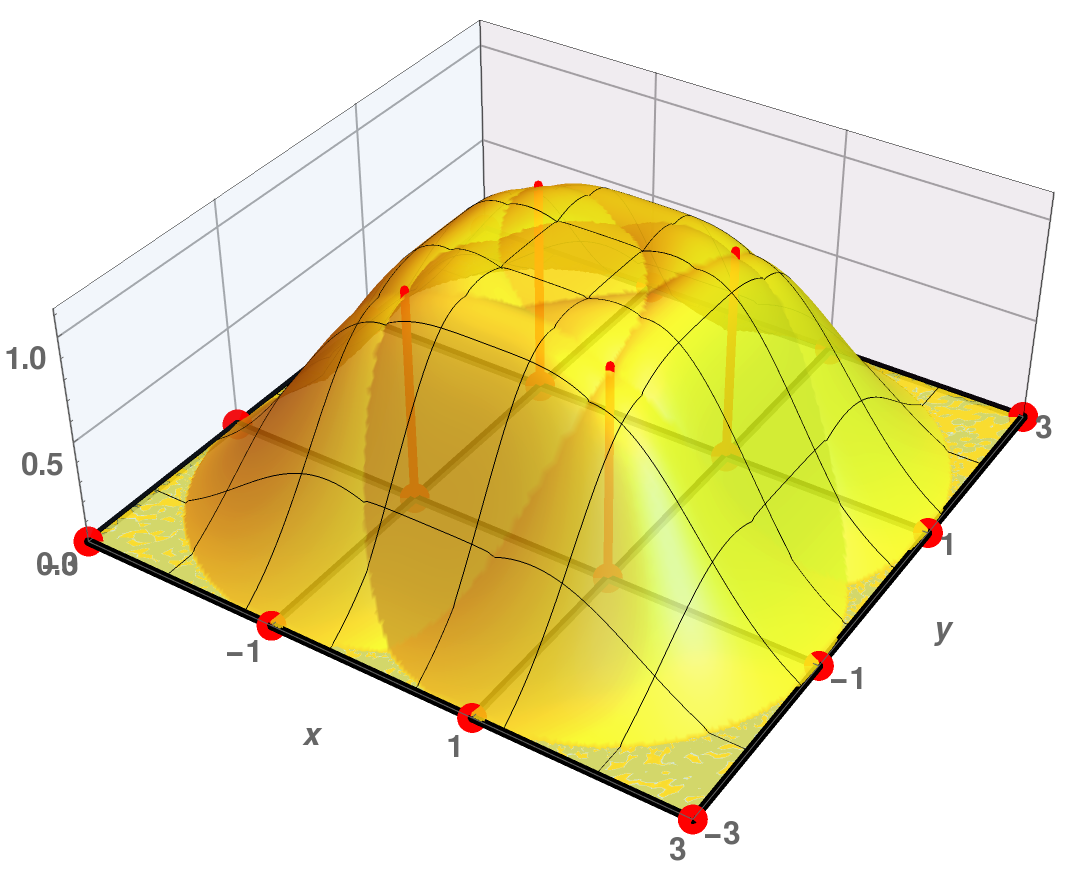
\includegraphics[width=0.94\textwidth]{Slike/sumOfNodeFs.png}
        \vspace{6mm}
        \caption{}
    \end{subfigure}
    \begin{subfigure}[b]{0.48\textwidth}
        \centering
        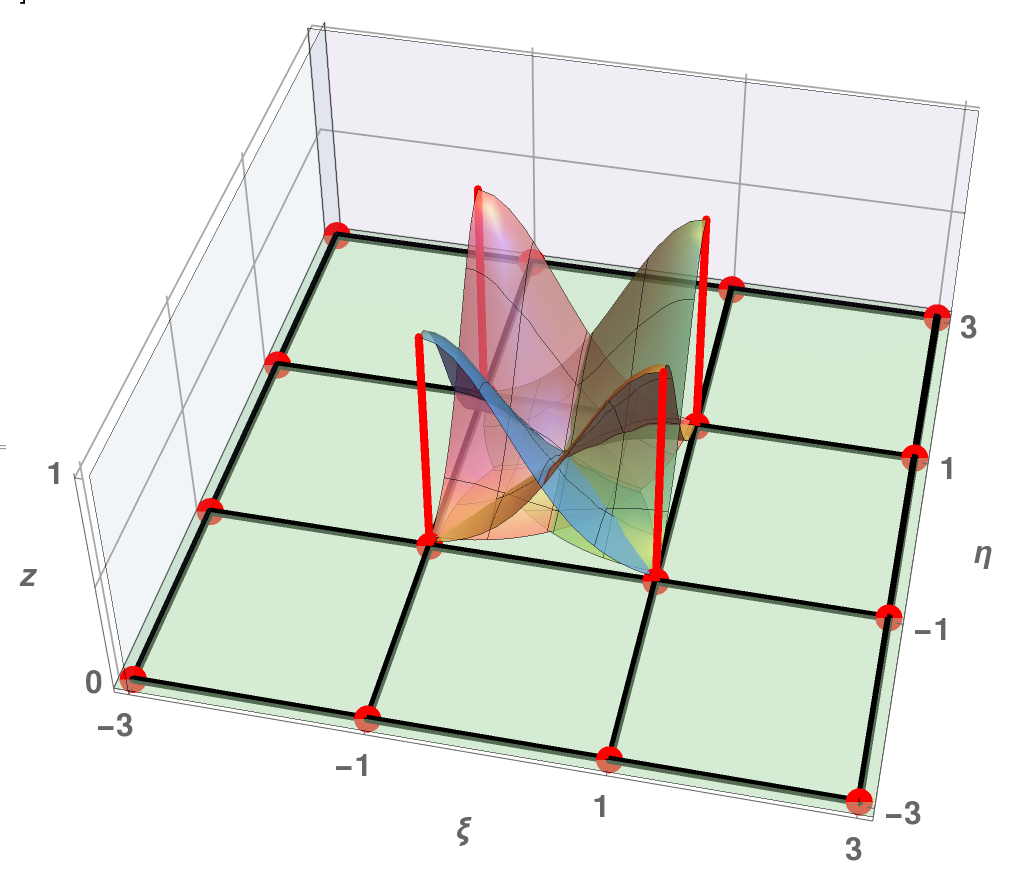
\includegraphics[width=0.94\textwidth]{Slike/undeformedShapeFsFar.png}
        \caption{}
    \end{subfigure}
    \caption{(a) vsota vozliščnih funkcij s slike \ref{fig:regionAndNodeFunctions}b in (b) elementarne funkcije, ki pripadajo elementu 5.}
    \label{fig:sumAndShapeFunctions}
\end{figure}

\begin{figure}[ht]
    \centering
    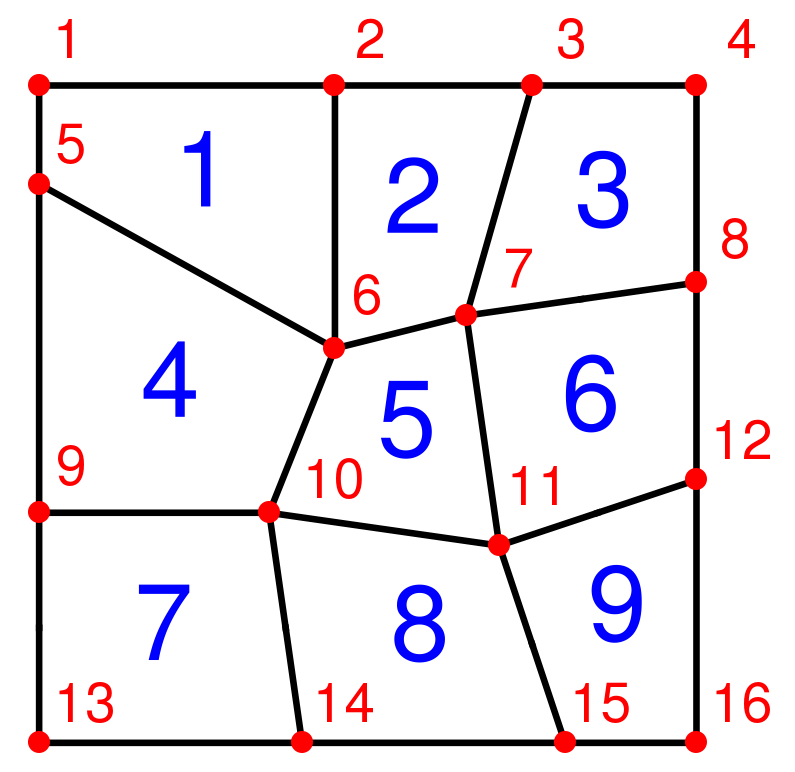
\includegraphics[height=80mm]{Slike/deformedRegion.png}
\end{figure}

\begin{figure}[ht]
    \begin{subfigure}[b]{0.48\textwidth}
        \centering
        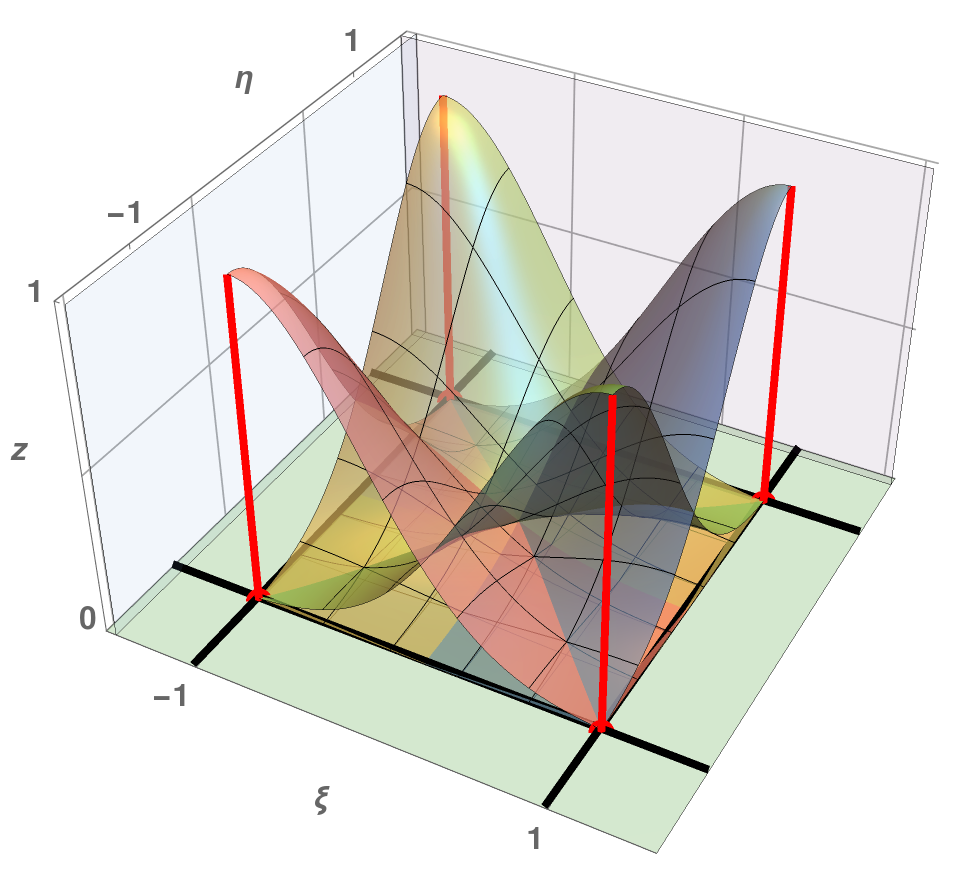
\includegraphics[width=0.94\textwidth]{Slike/undeformedShapeFs.png}
        \vspace{6mm}
        \caption{}
    \end{subfigure}
    \begin{subfigure}[b]{0.48\textwidth}
        \centering
        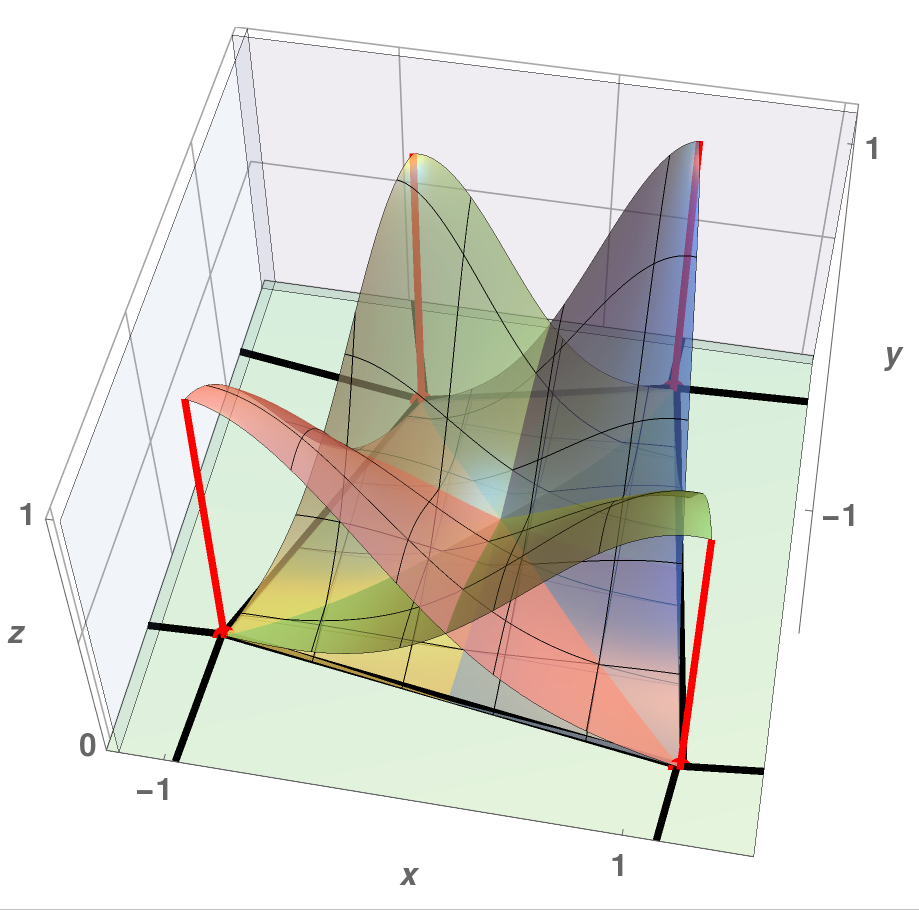
\includegraphics[width=0.94\textwidth]{Slike/deformedShapeFs.png}
        \caption{}
    \end{subfigure}
    \caption{}
    \label{fig:shapeFs}
\end{figure}

še vedno  Z natančno analitično izpeljavo se prebijemo do izjave \eqref{eq:LsfemVariationalStatement}, od tod dalje pa moramo iskanje funkcije $\mathbf{u(x)}$ z neskončno prostostnimi stopnjami poenostaviti v iskanje funkcije s končnim številom prostostnih stopenj $N$. 

Skozi oči \texttt{FI} je $\ket{\Phi_i}$ eden izmed baznih vektorjev v razvoju vektorja $\ket{v}$, $v_i$ pa pripadajoča komponenta.
V jeziku funkcionalne analize (\texttt{FI}) pravimo, da smo omejili funkcijski prostor.

nadaljujemo z diskretizacijo problema, to je, pretvorbo na sistem $N$ algebrajskih enačb. Ta korak je enak pri vseh različicah \texttt{FEM}. Funkcije na domeni $\Omega$ imajo neskončno štveilo prostostnih stopenj. 
\begin{equation}
    u_i(\mathbf{x}) = \sum_{a = 1}^N \Phi^{a0} u^{a0}_i
\end{equation}

Mreža je v tem šolskem primeru strukturirana, kar pomeni, da je razporeditev elementov Kartezična. Mreža je lahko pri \texttt{FEM} tudi nestrukturirana, kar je ena izmed prednosti metode.

Potem omejimo Diskretizacija problema 

Galerkin, Najmanših kvadratov \cite{JiangB-LSFEM}
Basic lemma of variational principles: Temeljni lema variacijskih načel.